\documentclass[aspectratio=169]{beamer}

% ---------------------------------------------------------------------------
% Projet final MongoDB — E-Commerce
% Compilation : pdflatex presentation.tex  (ou : make)
% ---------------------------------------------------------------------------

\usetheme{Madrid}
\usecolortheme{seahorse}
\usepackage[utf8]{inputenc}
\usepackage[T1]{fontenc}
\usepackage[french]{babel}
\usepackage{listings}
\usepackage{xcolor}
\usepackage{booktabs}
\usepackage{tikz}
\usetikzlibrary{positioning, arrows.meta}

% --- couleurs MongoDB ---
\definecolor{mongogreen}{HTML}{00684A}
\definecolor{mongoleaf}{HTML}{13AA52}
\definecolor{codebg}{HTML}{F4F6F5}
\setbeamercolor{structure}{fg=mongogreen}
\setbeamercolor{frametitle}{bg=mongogreen, fg=white}

% --- style code ---
\lstdefinestyle{mongo}{
  basicstyle=\ttfamily\scriptsize,
  backgroundcolor=\color{codebg},
  keywordstyle=\color{mongogreen}\bfseries,
  stringstyle=\color{orange!80!black},
  commentstyle=\color{gray}\itshape,
  numberstyle=\tiny\color{gray},
  showstringspaces=false,
  breaklines=true,
  frame=single,
  rulecolor=\color{mongoleaf},
  keywords={db, find, aggregate, insertOne, insertMany, updateOne, updateMany, deleteOne, deleteMany, createIndex, sort, limit, skip, match, group, lookup, unwind, project, sum, avg},
}
\lstset{style=mongo}

\title[E-Commerce MongoDB]{Application E-Commerce avec MongoDB}
\subtitle{Projet final — Formation MongoDB}
\author{Alexandre REY, Shayaan SHAKHUN, Prince ESSANI, Benjamin VARENNE}
\date{18 juin 2026}

\begin{document}

% ===========================================================================
\begin{frame}\titlepage\end{frame}

\begin{frame}{Sommaire}\tableofcontents\end{frame}

% ===========================================================================
\section{Présentation de l'équipe}
\begin{frame}{Présentation de l'équipe}
  \begin{columns}
    \begin{column}{0.55\textwidth}
      \begin{itemize}
        \item \textbf{Alexandre REY} — Backend \& API (FastAPI)
        \item \textbf{Shayaan SHAKHUN} — Modélisation MongoDB \& agrégations
        \item \textbf{Prince ESSANI} — Frontend (SPA Bootstrap)
        \item \textbf{Benjamin VARENNE} — Données de test \& déploiement
      \end{itemize}
      \vspace{1em}
      
    \end{column}
    \begin{column}{0.45\textwidth}
      \begin{block}{Organisation}
        \begin{itemize}
          \item Dépôt GitHub partagé
          \item Cluster MongoDB Atlas commun
          
        \end{itemize}
      \end{block}
    \end{column}
  \end{columns}
\end{frame}

% ===========================================================================
\section{Architecture de la solution}
\begin{frame}{Architecture de la solution}
  \centering
  \begin{tikzpicture}[
      node distance=1.4cm and 2.2cm,
      box/.style={draw, rounded corners, minimum width=2.6cm, minimum height=1.1cm, align=center, thick},
      arrow/.style={-{Stealth}, thick}
    ]
    \node[box, fill=mongoleaf!15] (front) {Frontend\\\footnotesize HTML/JS + Bootstrap};
    \node[box, fill=blue!10, right=of front] (api) {Backend\\\footnotesize FastAPI (Python)};
    \node[box, fill=mongogreen!20, right=of api] (db) {MongoDB Atlas\\\footnotesize Cluster cloud};

    \draw[arrow] (front) -- node[above, font=\scriptsize] {REST / JSON} (api);
    \draw[arrow] (api) -- node[above, font=\scriptsize] {PyMongo} (db);
    \draw[arrow, dashed] (api) to[bend right=30] node[below, font=\scriptsize] {réponses} (front);
    \draw[arrow, dashed] (db) to[bend left=30] node[below, font=\scriptsize] {documents} (api);
  \end{tikzpicture}

  \vspace{1em}
  \begin{itemize}
    \item Architecture 3 tiers : présentation, logique métier, persistance.
    \item Le backend expose une API REST consommée par le frontend.
    \item Toutes les opérations de données passent par PyMongo vers Atlas.
  \end{itemize}
\end{frame}

% ===========================================================================
\section{Technologies utilisées}
\begin{frame}{Description des technologies utilisées}
  \begin{columns}[t]
    \begin{column}{0.33\textwidth}
      \begin{block}{Frontend}
        \begin{itemize}\footnotesize
          \item HTML5 / JavaScript
          \item Bootstrap 5
          \item Fetch API (SPA)
        \end{itemize}
      \end{block}
    \end{column}
    \begin{column}{0.33\textwidth}
      \begin{block}{Backend}
        \begin{itemize}\footnotesize
          \item Python 3.12
          \item FastAPI + Uvicorn
          \item PyMongo
          \item Pydantic (validation)
        \end{itemize}
      \end{block}
    \end{column}
    \begin{column}{0.33\textwidth}
      \begin{block}{Base de données}
        \begin{itemize}\footnotesize
          \item MongoDB Atlas
          \item Cluster répliqué
          \item 10 collections
          \item Index ciblés
        \end{itemize}
      \end{block}
    \end{column}
  \end{columns}
  \vspace{1em}
  \centering\footnotesize
  Outils : Git/GitHub (versioning), MongoDB Compass (visualisation), VS Code.
\end{frame}

% ===========================================================================
\section{Schéma de la base de données}
\begin{frame}{Schéma de la base de données MongoDB}
  \centering
  % Diagramme entité-relation généré avec Mermaid (diagrams/db_schema.mmd)
  % puis exporté en PDF :  mmdc -i db_schema.mmd -o db_schema.pdf --pdfFit -t neutral
  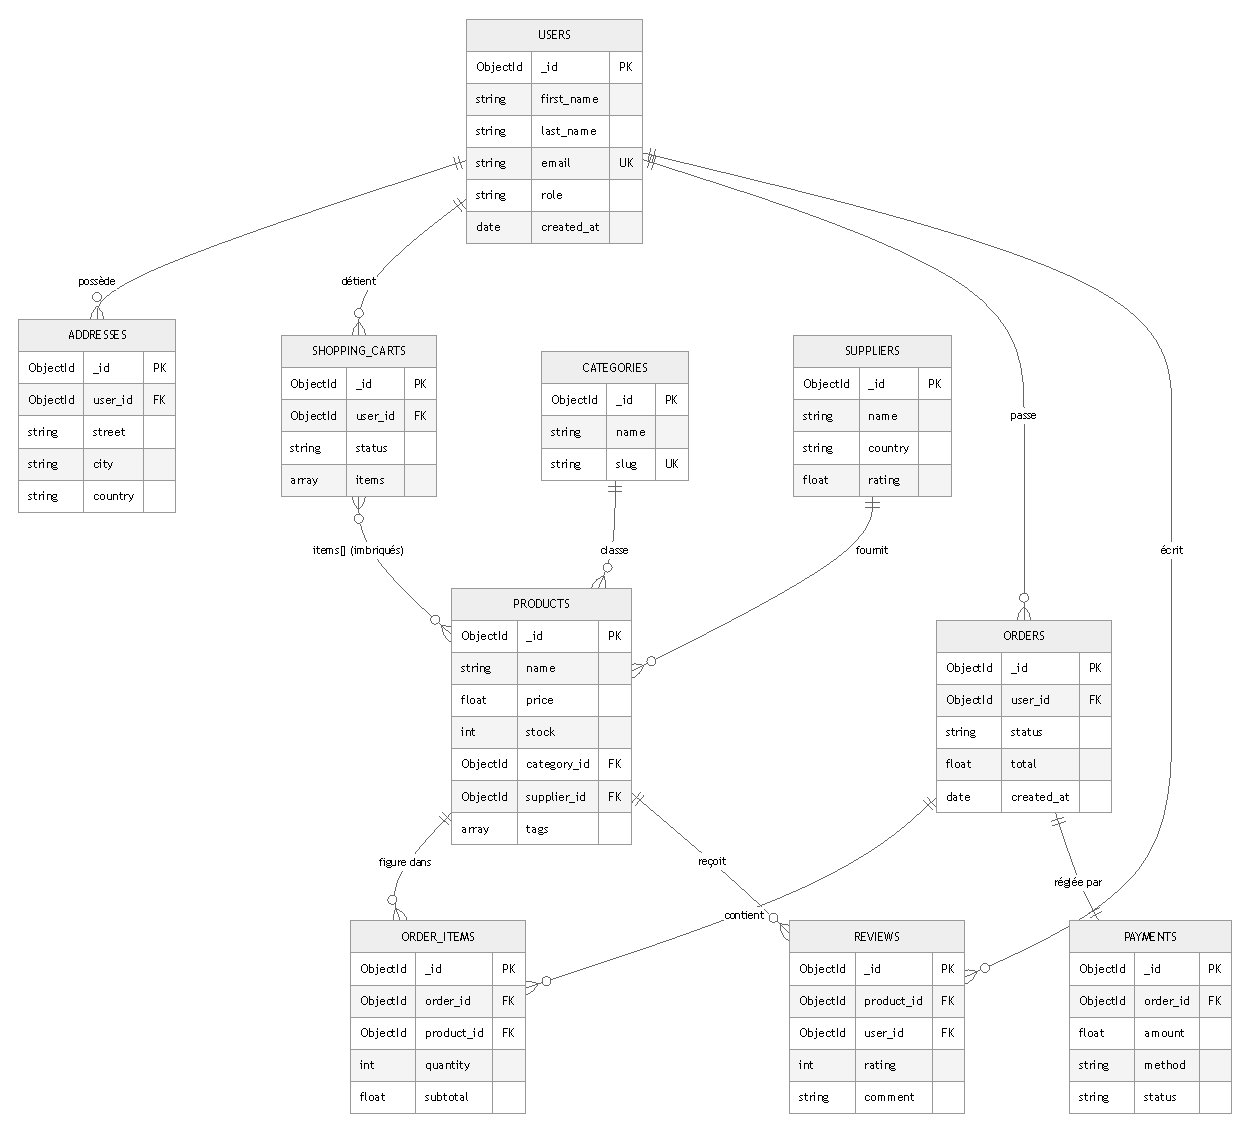
\includegraphics[width=\textwidth, height=0.78\textheight, keepaspectratio]{diagrams/db_schema.pdf}

  \vspace{0.4em}
  \footnotesize \texttt{PK} clé primaire, \texttt{FK} référence (\texttt{ObjectId}), \texttt{UK} clé unique.
\end{frame}

% ===========================================================================
\section{Description des collections}
\begin{frame}{Description des collections (10 collections)}
  \centering\scriptsize
  \begin{tabular}{@{}l l l@{}}
    \toprule
    \textbf{Collection} & \textbf{Rôle} & \textbf{Liens (références)} \\
    \midrule
    users          & Clients et admins               & — \\
    categories     & Catégories de produits          & — \\
    suppliers      & Fournisseurs                    & — \\
    products       & Catalogue produits              & category\_id, supplier\_id \\
    addresses      & Adresses de livraison           & user\_id \\
    shopping\_carts & Paniers ouverts (items intégrés) & user\_id, product\_id \\
    orders         & Commandes                       & user\_id \\
    order\_items    & Lignes de commande              & order\_id, product\_id \\
    payments       & Paiements (simulation)          & order\_id \\
    reviews        & Avis clients                    & product\_id, user\_id \\
    \bottomrule
  \end{tabular}

  \vspace{0.8em}
  \footnotesize Minimum 10 documents par collection — données cohérentes générées via \texttt{seed.py}.
\end{frame}

\begin{frame}[fragile]{Exemple de document — \texttt{products}}
\begin{lstlisting}
{
  "_id": ObjectId("..."),
  "name": "UltraBook Pro 14",
  "description": "Ordinateur portable ultra-fin...",
  "price": 1299.00,
  "stock": 42,
  "category_id": ObjectId("...electronics..."),
  "supplier_id": ObjectId("...supplier..."),
  "tags": ["premium", "bestseller"],
  "created_at": ISODate("2026-02-01T10:00:00Z")
}
\end{lstlisting}
  \footnotesize Modélisation mixte : \textbf{références} (catégorie, fournisseur) et \textbf{imbrication} (tableau \texttt{tags}, items du panier).
\end{frame}

% ===========================================================================
\section{Fonctionnalités}
\begin{frame}{Démonstration des fonctionnalités principales}
  \begin{columns}
    \begin{column}{0.5\textwidth}
      \textbf{Côté client}
      \begin{itemize}\footnotesize
        \item Catalogue avec filtres (prix, catégorie, stock, recherche)
        \item Fiche produit + avis clients
        \item Panier (ajout, suppression, total)
        \item Passage de commande + paiement simulé
        \item Historique des commandes
      \end{itemize}
    \end{column}
    \begin{column}{0.5\textwidth}
      \textbf{Côté gestion}
      \begin{itemize}\footnotesize
        \item Tableau de bord (KPI)
        \item Revenu par catégorie
        \item Top produits / top clients
        \item Stock faible par fournisseur
        \item CRUD complet via l'API
      \end{itemize}
    \end{column}
  \end{columns}
\end{frame}

% ===========================================================================
\section{Commandes MongoDB}
\begin{frame}[fragile]{Commandes MongoDB — Insertion \& recherche}
\begin{lstlisting}
// Insertion
db.users.insertOne({ first_name: "Ada", role: "customer" })
db.products.insertMany([ { name: "A" }, { name: "B" } ])

// Recherche + filtres avancés
db.products.find({ price: { $gte: 50, $lte: 300 } })
db.products.find({ $or: [ { tags: "sale" }, { stock: 0 } ] })
db.products.find({ name: { $regex: "pro", $options: "i" } })

// Projection + tri + pagination
db.products.find({}, { _id: 0, name: 1, price: 1 })
           .sort({ price: -1 }).skip(5).limit(5)
\end{lstlisting}
\end{frame}

\begin{frame}[fragile]{Commandes MongoDB — Agrégations \& \texttt{\$lookup}}
\begin{lstlisting}
// Revenu par categorie : order_items -> products -> categories
db.order_items.aggregate([
  { $lookup: { from: "products", localField: "product_id",
               foreignField: "_id", as: "p" } },
  { $unwind: "$p" },
  { $lookup: { from: "categories", localField: "p.category_id",
               foreignField: "_id", as: "c" } },
  { $unwind: "$c" },
  { $group: { _id: "$c.name", revenue: { $sum: "$subtotal" } } },
  { $sort: { revenue: -1 } }
])
\end{lstlisting}
\end{frame}

\begin{frame}[fragile]{Commandes MongoDB — Mise à jour, suppression, index}
\begin{lstlisting}
// Mise a jour
db.products.updateOne({ _id: id }, { $set: { on_promo: true } })
db.products.updateOne({ _id: id }, { $inc: { stock: 10 } })
db.shopping_carts.updateOne({ ... }, { $push: { items: {...} } })

// Suppression
db.reviews.deleteOne({ _id: id })
db.demo.deleteMany({})

// Indexation
db.users.createIndex({ email: 1 }, { unique: true })
db.products.createIndex({ name: "text", description: "text" })
db.products.find({ price: { $gte: 100 } }).explain()
\end{lstlisting}
  \footnotesize Démo live : \texttt{python backend/mongo\_demo.py}
\end{frame}

% ===========================================================================
\section{Difficultés \& solutions}
\begin{frame}{Difficultés rencontrées et solutions apportées}
  \centering\small
  \begin{tabular}{@{}p{5.5cm} p{6cm}@{}}
    \toprule
    \textbf{Difficulté} & \textbf{Solution} \\
    \midrule
    Sérialisation des \texttt{ObjectId} / dates en JSON & Fonction \texttt{serialize()} récursive côté backend \\
    Jointures entre collections & Pipelines d'agrégation avec \texttt{\$lookup} + \texttt{\$unwind} \\
    Cohérence stock / commande & Validation + \texttt{\$inc} atomique lors du checkout \\
    Accès partagé à la base & Cluster MongoDB Atlas + chaîne de connexion commune (\texttt{.env}) \\
    Travail collaboratif & Branches Git, pull requests, commits explicites \\
    \bottomrule
  \end{tabular}
\end{frame}

% ===========================================================================
\section{Conclusion}
\begin{frame}{Conclusion}
  \begin{itemize}
    \item Application E-Commerce \textbf{complète et fonctionnelle} : frontend, backend, MongoDB.
    \item Modélisation \textbf{cohérente} sur 10 collections liées.
    \item Couverture de \textbf{toutes les commandes} étudiées : CRUD, filtres, projections,
          tri, agrégations, \texttt{\$lookup}, indexation.
    \item Mise en place d'un \textbf{cluster partagé} et d'un \textbf{workflow Git} collaboratif.
  \end{itemize}
  \vspace{1em}
  \centering
  \Large\color{mongogreen}\textbf{Merci de votre attention !}
\end{frame}

\end{document}